\chapter{Kitaev}

\section{引言(未完成)}

在前面的章节里我们阐述了拓扑绝缘体在声学系统中的建模方法,并且以彩虹捕获为例说明了拓扑物态在声学应用中的潜力。除此之外,声学系统由于其宏观且易于实现的优势,成为观测新型量子拓扑物态的一个极佳的平台。这一章节里,我们以Kitaev链为例,在声学系统中实现了类似的结构,并且观测到了与马约拉纳零模类似的声学模态。

一方面,拓扑绝缘体具有多重拓扑相这一概念,吸引了众多研究者的广泛关注。在这以后,由于能够操控特殊的鲁棒电子态,这些电子态可抵御微观无序并支持无损能量传输,不同分类的拓扑绝缘体和拓扑超导体已被认为在量子技术方面具有重大潜力。尤其在拓扑量子计算领域,拓扑超导体有望为一类非阿贝尔任意子(也就是马约拉纳费米子)提供颇具价值的解决方案。这些马约拉纳费米子或许能以非局域且本质上无退相干的方式,将量子信息嵌入到量子计算机的实验合成中\cite{r31,r32,r33}。2001年,Kitaev提出了一个著名的模型——无自旋一维(1D)玩具模型,即无自旋p波超导N位链。该链能够支持未配对的端马约拉纳零模,这些零模在零能量处简并,而这是因为该系统在拓扑上具有非平凡的特性\cite{r4}。这一模型激发了大量关于在超流体和超导体中实现这种一维超导导线的研究\cite{r51,r52,r53,r54,r55,r56,r57,r58,r59,r510},但由于假设的无自旋费米子的缺乏以及p波配对的罕见性,要合成实际的Kitaev链,至今仍是一个持续存在的挑战。

另一方面,正如前文所述,经典波系统凭借其灵活性和可重构性,长期以来都被当作设计拓扑能带以及观测新奇量子现象的重要平台。但是,如果第三章采样的电声类比方法对拓扑绝缘体进行建模时,我们会发现这种方法亚波长尺度下无法构造两种符号相反的相互作用,即电子的正跳跃和负跳跃。而这是Kitaev提出它的玩具模型中必须的。因此,我们需要在声学系统里找到新的方法解决这个问题。值得关注的是,尽管Kitaev链的机械对应物已经在一些实验工作中有所研究\cite{C54},但在经典波系统中,能否实现具有可观测马约拉纳样零模的Kitaev链类似物,依旧是一个尚未解决的问题。

在本章中工作目的是将无自旋p波Kitaev链的概念从理论和实验两方面引入到声学系统中,并且在与原子系统的严格对应中,揭示了所创建的马约拉纳样零模的性质。与其他情况不同的是,在所设想的一维声线中,马约拉纳样零模无需额外的外场来利用超导近邻效应,而且能够通过声刺激直接被激发。通过巧妙地设计基于共振声学系统的Kitaev链的一维线网络,体声系统的拓扑相变以及未配对马约拉纳零模的出现都可以被精准观测到。更为重要的是,实验不仅验证了这种奇异拓扑态的存在,还展示了所呈现结构的“键盘”特性,也就是链的个体可调配置。这一特性使得在保持体隙的同时,能够对每个位点的拓扑进行局部控制,还可以对类似马约拉纳费米子的类似物进行灵活操控。这些令人着迷的结果意义非凡,很可能为经典波系统开辟新的途径,有助于在宏观尺度上对新型类量子材料展开探索。

本章内容如下:...

\section{Kitaev链模型简述}

\begin{figure}[h!]
    \centering
    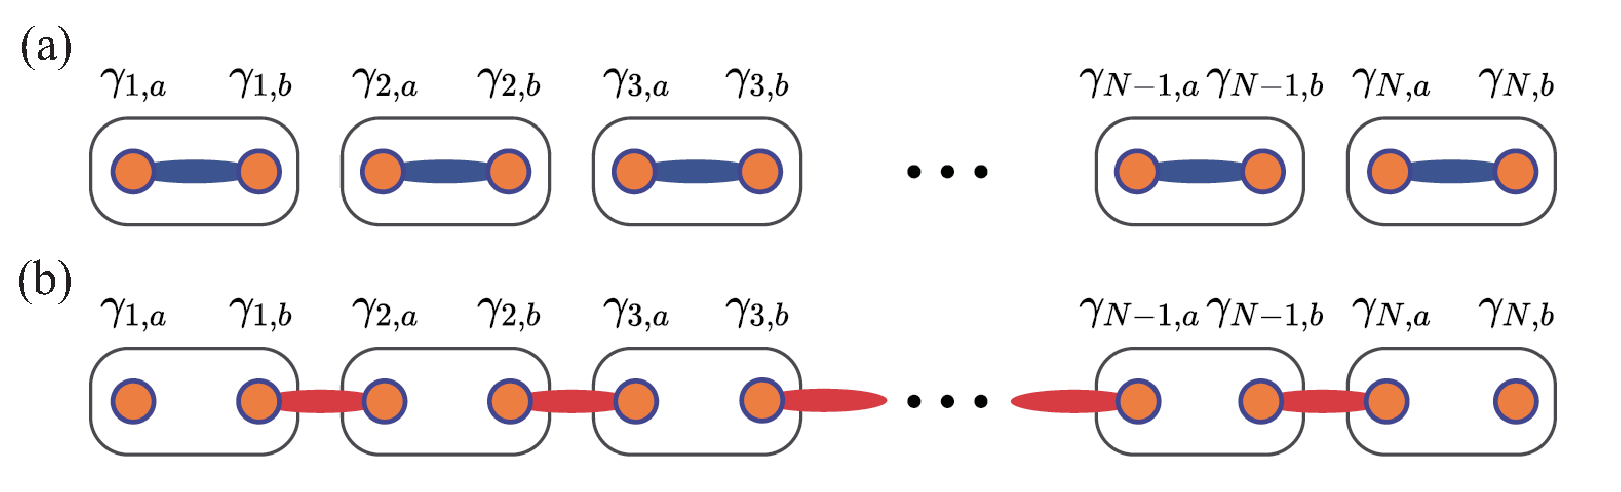
\includegraphics[width=1\textwidth]{images/fig5-1.eps} 
    \caption{(a) 极限情况$\Delta = t = 0$、$\mu \neq 0$下Kitaev链的图示 (b) $\Delta = t \neq 0$、$\mu = 0$下Kitaev链的图示。}
    \label{fig_5_1}
\end{figure}

在凝聚态物理研究中,探索超导体系的机制和拓扑特性是重要课题。2001年,Kitaev提出了无自旋p波超导N位链Kitaev链,在理论上实现马约拉纳零能模,并研究其非阿贝尔统计特性与拓扑保护机制。该模型最小哈密顿量$H$是研究其物理本质的关键,其形式最早在文献\cite{C54}中给出:
\begin{equation}\label{eq5-1}
    H = -\mu \sum_{n = 1}^{N} c_{n}^{\dagger} c_{n} - \sum_{n = 1}^{N - 1} (t c_{n + 1}^{\dagger} c_{n} + \Delta c_{n} c_{n + 1} + \text{H.c.})
\end{equation}
其中,各物理量意义明确。$t > 0$为最近邻跳跃强度,决定费米子在相邻晶格位点间跃迁的难易程度,影响体系粒子动力学行为;$\mu$是化学势,可调节体系粒子数分布,对系统热力学和电学性质有重要影响;$\Delta$是p波配对振幅,表征p波超导配对强度,是超导特性展现的关键因素。$c_{n}$作为第$n$个位点的无自旋费米子算符,是构建体系量子态的基本单元,通过对其运算可探究体系量子特性。

对该模型施加周期性边界条件后,可以分析其在动量空间的性质,得到Bogoliubov–de Gennes哈密顿量,其可写为:
\begin{equation}\label{eq5-2}
    H = \frac{1}{2} \sum_{k} C_{k}^{\dagger} \mathcal{H}(k) C_{k},
\end{equation}
其中,$C_{k}^{\dagger} = [c_{k}^{\dagger}, c_{-k}^{\dagger}]$,将正、负动量的费米子产生算符关联起来;$\mathcal{H}(k) = (-2t \cos k - \mu) \tau_{z} + 2\Delta \sin k \tau_{y}$,$\tau$为泡利矩阵,与体系动量相关项结合。对$\mathcal{H}(k)$进行对角化处理,可得到体能量本征值:
\begin{equation}\label{eq5-3}
    E(k) = \pm \sqrt{(2t \cos k + \mu)^{2} + 4\Delta^{2} \sin^{2} k},
\end{equation}
该表达式是理解体系能量结构的关键。当$\vert \mu \vert = 2t$时,在$k = 0$处发生体隙闭合,这是体系拓扑性质改变的重要信号,表明拓扑相变的临界点。在临界点附近,体系电子态密度、输运性质等物理性质会发生急剧变化,是探索模型拓扑性质与相关参数设置的核心。

在凝聚态物质系统中,电子在特定条件下对应成对的马约拉纳费米子。但Kitaev模型的独特之处在于,其关键的未成对马约拉纳费米子可通过哈密顿量以特殊方式实现。为理解链中拓扑相变及未成对马约拉纳费米子的出现,引入马约拉纳算符$\gamma_{n,a}$和$\gamma_{n,b}$(其中$\gamma_{n,\alpha} = \gamma_{n,\alpha}^{\dagger}$)替换无自旋费米子$c_{n}$,替换关系为$c_{n} = (\gamma_{n,a} - i\gamma_{n,b}) / 2$。通过替换,式\Ref{eq5-1}可重写为:
\begin{equation}\label{eq5-4}
    H = \frac{i}{2} \left\{ \sum_{n = 1}^{N - 1} [(-\Delta - t) \gamma_{n,b} \gamma_{n + 1,a} + (-\Delta + t) \gamma_{n + 1,b} \gamma_{n,a}] + \mu \sum_{n = 1}^{N} \gamma_{n,a} \gamma_{n,b} \right\}.
\end{equation}
为理解此式,从两个极限情况分析。第一种情况如图\ref{fig_5_1}(a),设$\Delta = t = 0$且$\mu \neq 0$,此时哈密顿量$H$简化为$H = (i / 2) \mu \sum_{n = 1}^{N} \gamma_{n,a} \gamma_{n,b}$。这表明马约拉纳模式$\gamma_{n,a}$和$\gamma_{n,b}$在同一位置成对,体系处于平庸相。在平庸相中,体系拓扑性质平庸,不存在特殊拓扑保护的量子态,物理性质可用传统凝聚态理论解释。

第二种极限情况如图\ref{fig_5_1}(b),当$\Delta = t$且$\mu = 0$时,哈密顿量变为$H = it \sum_{n = 1}^{N - 1} \gamma_{n,b} \gamma_{n + 1,a}$。这表明马约拉纳费米子从相邻位点成对,使得$\gamma_{1,a}$和$\gamma_{N,b}$未成对。由于体系的粒子 - 空穴对称性,这两个未成对马约拉纳费米子在零能量处形成端马约拉纳模式简并。这种零能量简并态稳定性高,受拓扑保护。同时,波函数对$[1, 0]^T$和$[0, 1]^T$在高对称点处的反转也佐证了拓扑相变的发生。综上,$\vert \mu \vert < 2t$表示体系处于具有部分填充能带对的非平庸超导态,具有丰富拓扑性质和独特量子特性,如存在受拓扑保护的边缘态;而$\vert \mu \vert > 2t$对应无马约拉纳费米子出现的平庸拓扑,此时体系物理性质与常规非拓扑超导体系相似,拓扑效应可忽略。 

\section{基于$P_z$模式的声学哈密顿量}

\begin{figure}[h!]
    \centering
    \includegraphics[width=1\textwidth]{images/fig5-2.eps} 
    \caption{(a) 声学Kitaev链的示意图。(b) 其中所展示链中声学参数的详细定义。青色虚线分别表示有效面积$S'$,而灰色线分别表示密封的声学边界。}
    \label{fig_5_2}
\end{figure}

正如前文所述,设计Kitaev链需要能同时实现正负跳跃系数,而前面两章体积的电声类比方法无法实现。2020年,Qi等人提出利用腔体的$P_z$模来来设计正负跳跃系数的方法\cite{j10}。换句话说,如果在波长远大于腔体尺寸的情况下,腔体里的声场分布总是均匀的,因此两个腔体之间的导管无论如何连接,引入的相互作用总是相同的。然而,利用$P_z$模态(即长腔体在z方向存在一个驻波的模态,如图\ref{fig_5_2(a)插图}),两个腔体之间的导管采用不同连接方式时,由于腔体声压本身在z方向存在声场分布,因此不同的连接方式引入的相互作用可以不同。在这里,我们详细补充描述了他们提出结构的声学理论建模,并应用在我们的Kitaev链的设计中。

我们为了实现如式\ref{eq5-4}的Kitaev链,设计了如图\ref{fig_5_2}(a)所示的声学结构。这个周期结构的晶格常数为\(a\),每个晶胞由两个单独的长方体声学腔组成,其长度和宽度分别为\(w\)和高度\(h\)。晶胞通过四根弯曲的管子复杂地连接(在图\ref{fig_5_2}(a)中分别用红色、黄色、蓝色和绿色标记),这些管子具有相同的边长\(d\)和有效长度\(l_{1}^{t}\)、\(l_{2}^{t}\)、\(l_{1}^{\Delta}\)和\(l_{2}^{\Delta}\)。此外,两根额外的管子(分别用紫色和橙色标记),其长度\(l_{1}^{\mu}\)和\(l_{2}^{\mu}\)可调,分别与每个晶胞中的两个腔体相连。空气的声速和密度分别为\(c_{0}\)和\(\rho_{0}\),并且最外层的管子都用声学硬边界封闭。

为了展示Kitaev链的严格声学对应性,我们详细展示了这个结构的声学哈密顿量的推导过程。
我们从一个单声学腔开始,该腔体与单元腔中连接的管道相连,如图\ref{fig_5_2}(b)所示。我们假设单个全封闭的刚性边界腔体对应的经典格林函数定义为 \( G(\vec{r}, \vec{r}') \)。当考虑传播频率为$\omega$的声波处于特定模式(即$P_z$-模式,单个腔内声速势的归一化场分布为$\psi(\vec{r}) = \sqrt{2/(w^2h)}\sin(\pi r_z/h)$),我们认为整个结构的共振频率的变化量是小量,因此$G(\vec{r},\vec{r}')$可简化为只取$P_z$模式频率附近的项,即:
\begin{equation}\label{eq5-5}
    G(\vec{r},\vec{r}') = \sum_{j} \frac{c_0^2}{\omega_j^2 - \omega^2} \psi_j(\vec{r}')\psi_j(\vec{r}) \approx \frac{c_0^2}{\omega_0^2 - \omega^2} \psi^*(\vec{r}')\psi(\vec{r}),
\end{equation}
其中$\psi(\vec{r})$是在位置$\vec{r}$处的声速势,$\omega_0$是作为腔中驻波的$P_z$-偶极模式的本征频率。需要强调的是,当$\omega$接近$\omega_0$时,上述近似成立。相应地,腔中的声压场分布可引入为
\begin{equation}\label{eq5-6}
    p(\vec{r}) = -i\rho_0\omega \int_{\partial V} G(\vec{r},\vec{r}')v(\vec{r}')dS' \approx -\frac{i\rho_0c_0^2\omega}{\omega_0^2 - \omega^2} \psi(\vec{r}) \int_{\partial V} \psi^*(\vec{r}')v(\vec{r}')dS',
\end{equation}
其中$v(\vec{r}')$表示声速,$S'$表示腔的表面积。由于声硬边界条件下$v = 0$,式(S2)中的积分仅在管的端部不为零,因此有效面积可表示为$S' = 2S' + 2S^{\Delta} + S^{\mu}$,其中上标分别表示相应的管,如图\ref{fig_5_2}(b)中的虚线区域所示。相应地,我们现在引入下标$j$($j = 1,2$)来区分一个单胞中两个腔的参数,并且定义$\xi = [\xi_1,\xi_2]^T$为
\begin{equation}\label{eq5-7}
    \begin{split}
    \xi_1 & = \frac{p_1(\vec{r}_1)}{\psi_1(\vec{r}_1)} = -\frac{i\omega\rho_0c_0^2}{\omega_0^2 - \omega^2} \int_{\partial V_1} \psi^*(\vec{r}_1')v_1(\vec{r}_1')dS_1' \\
    & \approx \frac{i\rho_0c_0^2d^2}{2(\omega - \omega_0)} (-v_1'(0) \Psi_1^* - v_1^{\Delta}(0) \Psi_1^{*'} + v_1^1(l_1) e^{-ik\alpha} \Psi_1^{*'} + v_2^{\Delta}(l_2) e^{-ik\alpha} \Psi_2^{*'} - \sqrt{\frac{2}{V}}v_1^1), \\
    \xi_2 & = \frac{p_2(\vec{r}_2)}{\psi_2(\vec{r}_2)} = -\frac{i\omega\rho_0c_0^2}{\omega_0^2 - \omega^2} \int_{\partial V_2} \psi^*(\vec{r}_2')v_2(\vec{r}_2')dS_2' \\
    & \approx \frac{i\rho_0c_0^2d^2}{2(\omega - \omega_0)} (-v_2'(0) \Psi_2^* - v_2^{\Delta}(0) \Psi_2^{*'} + v_2^1(l_2) e^{-ik\alpha} \Psi_2^{*'} + v_1^{\Delta}(l_1) e^{-ik\alpha} \Psi_1^{*'} - \sqrt{\frac{2}{V}}v_2^1)
    \end{split}
\end{equation}
其中$V = w^2h$是腔的体积,$\overline{\Psi}_j^{m*}$是连接到第$j$个腔的第$m$根管端部的声速势平均值,由于所有管具有相同的横截面积和相同的腔的$r_z$,因此恰好满足关系$\overline{\Psi}_1 = \overline{\Psi}_2 = -\overline{\Psi}_1^{\Delta} = -\overline{\Psi}_2^{\Delta} = \overline{\Psi}$,从而有$|\overline{\Psi}_j^{m}| = |\overline{\Psi}|$。同时,值得注意的是,由于管的尺寸比腔小得多,该近似是可行的。根据这些结果,我们可以将声压用$\xi$表示为:
\begin{equation}
    \begin{split}
    p_j^{'}(0) & = \xi_j\overline{\Psi}_j \\
    p_j^{\Delta}(0) & = \xi_j\overline{\Psi}_j^{\Delta} \\
    p_j^{'}(l_j^{'}) & = e^{ika} \xi_j\overline{\Psi}_j \\
    p_1^{\Delta}(l_1^{\Delta}) & = e^{ika} \xi_2\overline{\Psi}_2^{\Delta}, \quad p_2^{\Delta}(l_2^{\Delta}) = e^{ika} \xi_1\overline{\Psi}_1^{\Delta} \\
    p_j^{\mu} & = \xi_j\sqrt{\frac{2}{V}}
    \end{split}
    \label{eq5-8}
\end{equation}
为了描绘出严格的对应关系,我们现在关注管的声学连接条件。我们认为结构内的声波以平面波传播,那么在一个单胞中第$j$个腔中的声压以及声速则具有以下形式:
\begin{equation}
    \begin{split}
    p_j^m(l) &= A_j^m e^{i\omega_0 l / c_0} + B_j^m e^{-i\omega_0 l / c_0}\\
    \rho_0 c_0 v_j^m(l) &= A_j^m e^{i\omega_0 l / c_0} - B_j^m e^{-i\omega_0 l / c_0}
    \end{split}
    \label{eq5-9}
\end{equation}
其中$m$表示$t$和$\Delta$。通过将$l = 0$和$l = l_j^m$代入方程\ref{eq5-8},很容易得到该关系:
\begin{equation}\label{eq5-10}
    i\rho_0 c_0\begin{bmatrix}v_j^m(0)\\v_j^m(l_j^m)\end{bmatrix}=\begin{bmatrix}\cot(\omega_0 l_j^m / c_0)&-\csc(\omega_0 l_j^m / c_0)\\\csc(\omega_0 l_j^m / c_0)&-\cot(\omega_0 l_j^m / c_0)\end{bmatrix}\begin{bmatrix}p_j^m(0)\\p_j^m(l_j^m)\end{bmatrix}
\end{equation}
对于一端封闭的附加管(用$\mu$标记),它满足以下关系:
\begin{equation}\label{eq5-11}
    v_j^{\mu} = \frac{p_j^{\mu}}{Z_j^{\mu}},
\end{equation}
其中$Z_j^{\mu}$是连接腔的端部的阻抗,当封闭端为声硬边界时,$Z_j^{\mu} = -i\rho_0 c_0\cot(\omega_0 l_j^{\mu} / c_0)$,而当为声软边界时,$Z_j^{\mu} = i\rho_0 c_0\tan(\omega_0 l_j^{\mu} / c_0)$。此外,通过将方程\ref{eq5-8}到\ref{eq5-11}代入方程\ref{eq5-7},以$\xi = [\xi_1,\xi_2]^T$表示的波函数方程可以写成矩阵形式为:
\begin{equation}\label{eq5-12}
    \omega \xi = (\mathcal{H}_0 + \mathcal{H}_a(k))\xi
\end{equation}
其中
\begin{equation}\label{eq5-13}
    \mathcal{H}_0 = 
    \begin{pmatrix}
    \omega_0 + \varepsilon_1 & 0 \\
    0 & \omega_0 + \varepsilon_2
    \end{pmatrix},
\end{equation}
\begin{equation}\label{eq5-14}
    \mathcal{H}_a(k) =
    \begin{pmatrix}
        \mu_1 + 2t_1\cos(ka) & \Delta_1 e^{ika} + \Delta_2 e^{-ika} \\
        \Delta_1 e^{-ika} + \Delta_2 e^{ika} & \mu_2 + 2t_2\cos(ka),
    \end{pmatrix},
\end{equation}
这里的参数表达式为
\begin{equation}\label{eq5-15}
    \begin{split}
    \varepsilon_1 &= \frac{c_0d^2|\overline{\Psi}|^2}{2}\left[2\cot\left(\frac{\omega_0l_1^t}{c_0}\right) + \cot\left(\frac{\omega_0l_1^{\Delta}}{c_0}\right) + \cot\left(\frac{\omega_0l_2^{\Delta}}{c_0}\right)\right] \\ \quad \\
    \varepsilon_2 &= \frac{c_0d^2|\overline{\Psi}|^2}{2}\left[2\cot\left(\frac{\omega_0l_2^t}{c_0}\right) + \cot\left(\frac{\omega_0l_2^{\Delta}}{c_0}\right) + \cot\left(\frac{\omega_0l_1^{\Delta}}{c_0}\right)\right]
    \end{split}
\end{equation}
    
\begin{equation}\label{eq5-16}
    t_1 = -\frac{c_0d^2|\overline{\Psi}|^2}{2}\csc\left(\frac{\omega_0l_1^t}{c_0}\right), \quad t_2 = -\frac{c_0d^2|\overline{\Psi}|^2}{2}\csc\left(\frac{\omega_0l_2^t}{c_0}\right),
\end{equation}
    
\begin{equation}\label{eq5-17}
    \Delta_1 = -\frac{c_0d^2|\overline{\Psi}|^2}{2}\csc\left(\frac{\omega_0l_1^{\Delta}}{c_0}\right), \quad \Delta_2 = -\frac{c_0d^2|\overline{\Psi}|^2}{2}\csc\left(\frac{\omega_0l_2^{\Delta}}{c_0}\right),
\end{equation}
    
\begin{equation}\label{eq5-18}
    \mu_1 = \frac{i\rho_0c_0^2d^2}{VZ_1^{\mu}}, \quad \mu_2 = \frac{i\rho_0c_0^2d^2}{VZ_2^{\mu}},
\end{equation}

需注意的是,一旦声学结构得以确定,所有定义清晰的参数均可直接计算。更重要的是,方程\ref{eq5-15}至\ref{eq5-18}表明,由$P_z$模式所描述的模型参数($t$、$\Delta$和$\mu$)是解耦的,这与前述共振声学系统中基频所描述的跃迁情况不同,正因如此,这些关键强度可独立设计。

更进一步,为构建一个严格的声学Kitaev链,需满足$l_1^t = l_2^t + h$,从而使得$t_1 = -t_2 = -t$;$l_1^{\Delta} = l_2^{\Delta} + h$,进而使得$\Delta_1 = -\Delta_2 = -\Delta$;以及$Z_1^{\mu} = -Z_2^{\mu}$,以此使得$\mu_1 = -\mu_2 = -\mu$。并且,这样的设置自然能确保$\varepsilon_1 = \varepsilon_2 = \varepsilon$。如此一来,方程\ref{eq5-13}和\ref{eq5-14}可化简为:
\begin{equation}\label{eq5-19}
    \mathcal{H}_0 = 
    \begin{pmatrix}
    \omega_0 + \varepsilon & 0 \\
    0 & \omega_0 + \varepsilon
    \end{pmatrix},
\end{equation}
\begin{equation}\label{eq5-20}
    \mathcal{H}_a(k) = 
    \begin{pmatrix}
    -\mu - 2t\cos(ka) & -2i\Delta\sin(ka) \\
    2i\Delta\sin(ka) & \mu + 2t\cos(ka)
    \end{pmatrix},
\end{equation}

由此,$\mathcal{H}_a(k)$是与Kitaev原文献中的哈密顿量完全一致\cite{r4},而$\mathcal{H}_0$仅对整个频谱的频移产生影响,并不影响系统的拓扑结构。至此,声学Kitaev链的哈密顿量\ref{eq5-20}与我们设计的结构通过以上推导完全对应,Kitaev模型中的所有参数在声学系统中的设计方法通过方程\ref{eq5-15}至\ref{eq5-18}全部给出。





\section{实际结构}

我们现在关注上述讨论的基塔耶夫链的声学对应物,晶格常数为\(a\)的一维线结构如图1(a)所示。这里每个晶胞由两个单独的长方体声学腔组成,其长度和宽度分别为\(w\)和高度\(h\)。晶胞通过四根弯曲的管子复杂地连接(在图1(a)中分别用红色、黄色、蓝色和绿色标记),这些管子具有相同的边长\(d\)和有效长度\(l_{1}^{t}\)、\(l_{2}^{t}\)、\(l_{1}^{\Delta}\)和\(l_{2}^{\Delta}\)。此外,两根额外的管子(分别用紫色和橙色标记),其长度\(l_{1}^{\mu}\)和\(l_{2}^{\mu}\)可调,分别与每个晶胞中的两个腔体相连。空气的声速和密度分别为\(c_{0}\)和\(\rho_{0}\),并且最外层的管子都用声学硬边界封闭。

为了合成类似的马约拉纳费米子,我们现在考虑在系统中以\(P_{z}\)模式传播的声波[图1(a)],它对应于频率为\(\omega_{0}\)的偶极驻波。相应地,第\(j\)个(\(j = 1,2\))每个晶胞腔体中的声速势的正态分布可以写为\(\psi_{j}(\vec{r}) = \sqrt{2 /(w^{2} h)} \sin(\pi r_{z} / h)\),其中\(r_{z}\)是\(\vec{r}\)在\(z\)方向的分量。进一步,通过定义参数\(\xi = [\xi_{1}, \xi_{2}]^{T}\),其中\(\xi_{j} = p_{j}(\vec{r}) / \psi_{j}(\vec{r})\)(\(p_{j}(\vec{r})\)是相应的声压),那么具有传播频率\(\omega\)的\(\xi\)表示的声场分布满足

\(\omega \xi = [\mathcal{H}_{0} + \mathcal{H}_{a}(k)] \xi\),\((4)\)

其中

\(\mathcal{H}_{0} = \begin{pmatrix} \omega_{0} + \epsilon_{1} & 0 \\ 0 & \omega_{0} + \epsilon_{2} \end{pmatrix}\),

\(\mathcal{H}_{a}(k) = \begin{pmatrix} \mu_{1} + 2t_{1} \cos(ka) & \Delta_{1} e^{ika} + \Delta_{2} e^{-ika} \\ \Delta_{1} e^{-ika} + \Delta_{2} e^{ika} & \mu_{2} + 2t_{2} \cos(ka) \end{pmatrix}\),\((5)\)

其中\(\epsilon_{1} = (c_{0} d^{2}|\vec{\psi}^{\prime}|^{2} / 2)[2 \cot(\omega_{0} l_{1}^{t} / c_{0}) + \cot(\omega_{0} l_{1}^{\Delta} / c_{0}) + \cot(\omega_{0} l_{1}^{\mu} / c_{0})]\)表示由连接到相应腔体的管子引起的总微扰,\(\epsilon_{2}\)具有相同形式但下标相反。关键的是,关键的对应关系被明确确定为\(t_{j} = -(c_{0} d^{2}|\vec{\psi}^{\prime}|^{2} / 2) \csc(\omega_{0} l_{j}^{t} / c_{0})\),\(\Delta_{j} = -(c_{0} d^{2}|\vec{\psi}^{\prime}|^{2} / 2) \csc(\omega_{0} l_{j}^{\Delta} / c_{0})\),以及\(\mu_{j} = i(\rho_{0} c_{0}^{2} d^{2}) /(w^{2} h Z_{j}^{\mu})\),其中\(|\vec{\psi}^{\prime}|\)表示\(\psi(\vec{r})\)在管子两端的平均值,\(Z_{j}^{\mu} = -i \rho_{0} c_{0} \cot(\omega_{0} l_{j}^{\mu} / c_{0})\)是额外管子的阻抗(见补充材料[50]的I节)。值得注意的是,所有参数自然解耦,振幅以及符号因此可以独立操纵。此外,一旦设置\(l_{1}^{t} = l_{2}^{t} + h\)和\(l_{1}^{\Delta} = l_{2}^{\Delta} + h\),我们得到\(\epsilon_{1} = \epsilon_{2}\),\(t_{1} = -t_{2}\),以及\(\Delta_{1} = -\Delta_{2}\),并立即发现\(\mathcal{H}_{a}(k)\)严格等同于\(\mathcal{H}(k)\)(在式(2)中),而\(\mathcal{H}_{0}\)仅在实践中贡献一个谱移。因此,基塔耶夫链最终可以在声学系统中实现。

根据上述讨论,我们现在设置\(w = 2.5\)厘米,\(h = 7.5\)厘米,\(d = 0.5\)厘米,\(l_{1}^{t} = 18.25\)厘米,\(l_{2}^{t} = 10.5\)厘米,\(l_{1}^{\Delta} = 18.95\)厘米,\(l_{2}^{\Delta} = 11.2\)厘米(因此\(l = 184\)和\(l^{\Delta} = 180\)),并通过仅控制\(l^{\mu}\)在声学基塔耶夫链中展示以下拓扑相变。图1(b) - 1(d)分别描绘了晶胞中\(\vert \mu \vert < 2t\)、\(\vert \mu \vert = 2t\)和\(\vert \mu \vert > 2t\)的过程,相应的理论和数值能带结构分别在图1(e) - 1(g)中给出,这为系统中的拓扑相变提供了良好的证据(见补充材料[50]的II节)。特别是,作为系统中关键的已识别拓扑特征,预计在基塔耶夫链的两端会出现一对不成对的马约拉纳零模式。两种极限情况下基塔耶夫链的图示分别在图2(a)和2(b)中给出,七个位点的声学对应物的能量谱分别在图2(c)和2(d)中给出。可以清楚地看到,与拓扑平凡时的完全体隙相比,在非平凡相中,两个简并的马约拉纳零模式恰好被钉扎在频率\(\omega_{0} + \epsilon\)处。关键的是,这种奇异模式的声场分布如图2(e)和2(f)所示,表明它们是不成对的。以下将详细进行实验。

\section{实验}

首先,我们考虑\(\vert \mu \vert = 2t\)时的能隙闭合条件。经过线性展开后,哈密顿量\(\mathcal{H}(k)\)具有如下形式:

\(\mathcal{H}(k) = m\tau_{z} + 2\Delta k\tau_{y}\),\((6)\)

其中\(m = -\mu - 2t\)是质量项。结果是,\(m = 0\)表示一个临界点,\(m\)的正负号因此表示不同的拓扑相,这提醒我们马约拉纳样零模式可以作为具有不同拓扑的两个畴之间的畴壁态出现。如图3(a)所示,我们构建了一个具有六个平凡(\(m > 0\))和六个非平凡(\(m < 0\))晶胞的声学样品作为畴壁。为了识别马约拉纳零模式,每个位点腔体都开有一个孔(当不在测量时用声学密封),并在样品外靠近畴壁处放置一个宽带声学激励源。图3(b)显示了测量的强度谱,很明显在约2430Hz处有一个光谱孤立的峰值,这恰好对应于图2(b)中预测的马约拉纳零模式频率。同时,马约拉纳样零模式的测量空间分布如图3(c)所示,展示了马约拉纳波函数的局域性(见补充材料[50]的III节)。因此,这些实验结果证实了声学基塔耶夫链中存在经典的马约拉纳样零模式。

最后,在理论模型中,只要化学势得到调节,马约拉纳费米子就可以被操控,这为“声学系统”带来了灵感。我们进行了基塔耶夫“键盘”的实验,以验证声学马约拉纳样零模式的准粒子特性[10]。由于在所呈现的结构中\(\mu\)和\(t\)是解耦的,我们现在定义一个拓扑相为“开(ON)”,平凡相为“关(OFF)”,如图4(a)所示,并且可以通过调节\(l^{\mu}\)轻松切换门(见图4(b))。相应地,给定的门可以被局部控制,这允许类似马约拉纳费米子被创建、传输和自由融合。图4(c)概述了一个跨越12个位点的基塔耶夫“键盘”的设置,这对应于三个独立实验,测量的空间强度分布分别在图4(d) - 4(f)中给出。因此,一个不成对的马约拉纳样零模式从位点2被驱动到位点6(见图4(d)),并且声学模式可以在传输过程中要么融合为一个有限能量模式(图4(e)中的位点5和位点8),要么通过控制门在位点5和位点8处被创建(见图4(f))(见补充材料[50]的IV节)。测量结果直接表明声学马约拉纳样零模式可以充当准粒子。此外,与一些现有的模型(如声学Su - Schrieffer - Heeger模型)相比,在我们的模型中只需要调节管子的长度,并且我们可以在单个样品中轻松实现各种功能。这一优势源于基塔耶夫链,它只需要调节化学势来操控马约拉纳费米子。

\section{小结}